%
% Slide template for the FreeBSD Developer Summit.
% Take it or leave it :-)
%
% It requires LaTeX and LaTeX Beamer [1] to compile.
% pdfLaTeX is recommended for compilation as it produces
% PDF file immediately.
%
% $ pdflatex some.latex
%
%
% It is also recommended to convert images to PDF
% by using ImageMagick ("convert") before including them.
%
% [1] http://latex-beamer.sourceforge.net
%

\documentclass{beamer}

\usepackage{url}
\usepackage[english]{babel}
%%\usepackage{verbatim}
%%\usepackage{times}
\usepackage{ubuntu}
\usepackage{graphicx}
\usepackage{listings}
\usepackage{mathtools}
\usepackage{color}
\usepackage{tikz}
\usetikzlibrary{arrows,shapes}

\mode<presentation>
{
  \definecolor{beamer@gker}{rgb}{0.8,0.0,0.0}
  \setbeamercolor*{structure}{fg=beamer@gker}
  \logo{
\includegraphics[scale=0.5]{logo.pdf}}
  \renewcommand{\sfdefault}{ubuntu}
}

\setbeamertemplate{footline}[text line]{%
  \parbox{\linewidth}{\vspace*{-8pt}
  \hfill
  \insertshortauthor
  \hfill
  \insertframenumber\ of \inserttotalframenumber}}
\setbeamertemplate{navigation symbols}{}

\definecolor{light-gray}{gray}{0.60}

\title{FreeBSD package management system}
\author{Vsevolod Stakhov \\ \url{vsevolod@FreeBSD.org}}
\institute{
\includegraphics[scale=0.5]{logo.pdf}}
\date{BSDCan \
May 17, 2014}

\begin{document}

\begin{frame}[plain]
  \titlepage
\end{frame}

%%\begin{frame}
%%\frametitle{Disadvantages of the ports}
%%The ports are very mature and well designed system, however, there are some
%%disadvantages in managing a system merely using the ports.
%%\begin{itemize}
%%  \item The ports use \texttt{make} that cannot handle complex packages
%%  relationships
%%  \item Complicated upgrade procedure (hard to keep up-to-date)
%%  \item Hard to migrate between releases
%%  \item Long build time
%%\end{itemize}
%%\end{frame}

\begin{frame}
\frametitle{What is pkg}
Pkg (previously pkgng) is the binary package management system written for
FreeBSD.
\begin{itemize}
  \item Binary packages management
  \item Replaces old \texttt{pkg\_*} tools
  \item Uses central sqlite3 based storage
  \item Provides the comprehensive toolset for binary packages management
\end{itemize}
\end{frame}

\begin{frame}
\frametitle{Pkg development goals}
The main goal of pkg is to simplify system management tasks.
\begin{itemize}
  \item Easy install, remove and upgrade of binary packages
  \item Integration with the ports
  \item Automatic resolving of dependencies and conflicts
  \item Provide secure package management tool
  \item Encourage users to install software from binary packages
  \item<2-> \ldots but do not prevent users from building custom packages using
  the ports
\end{itemize}
\end{frame}


%%\begin{frame}[fragile]
%%\frametitle{Ports before pkg}
%%\begin{figure}[h!]
%%  \centering
%%  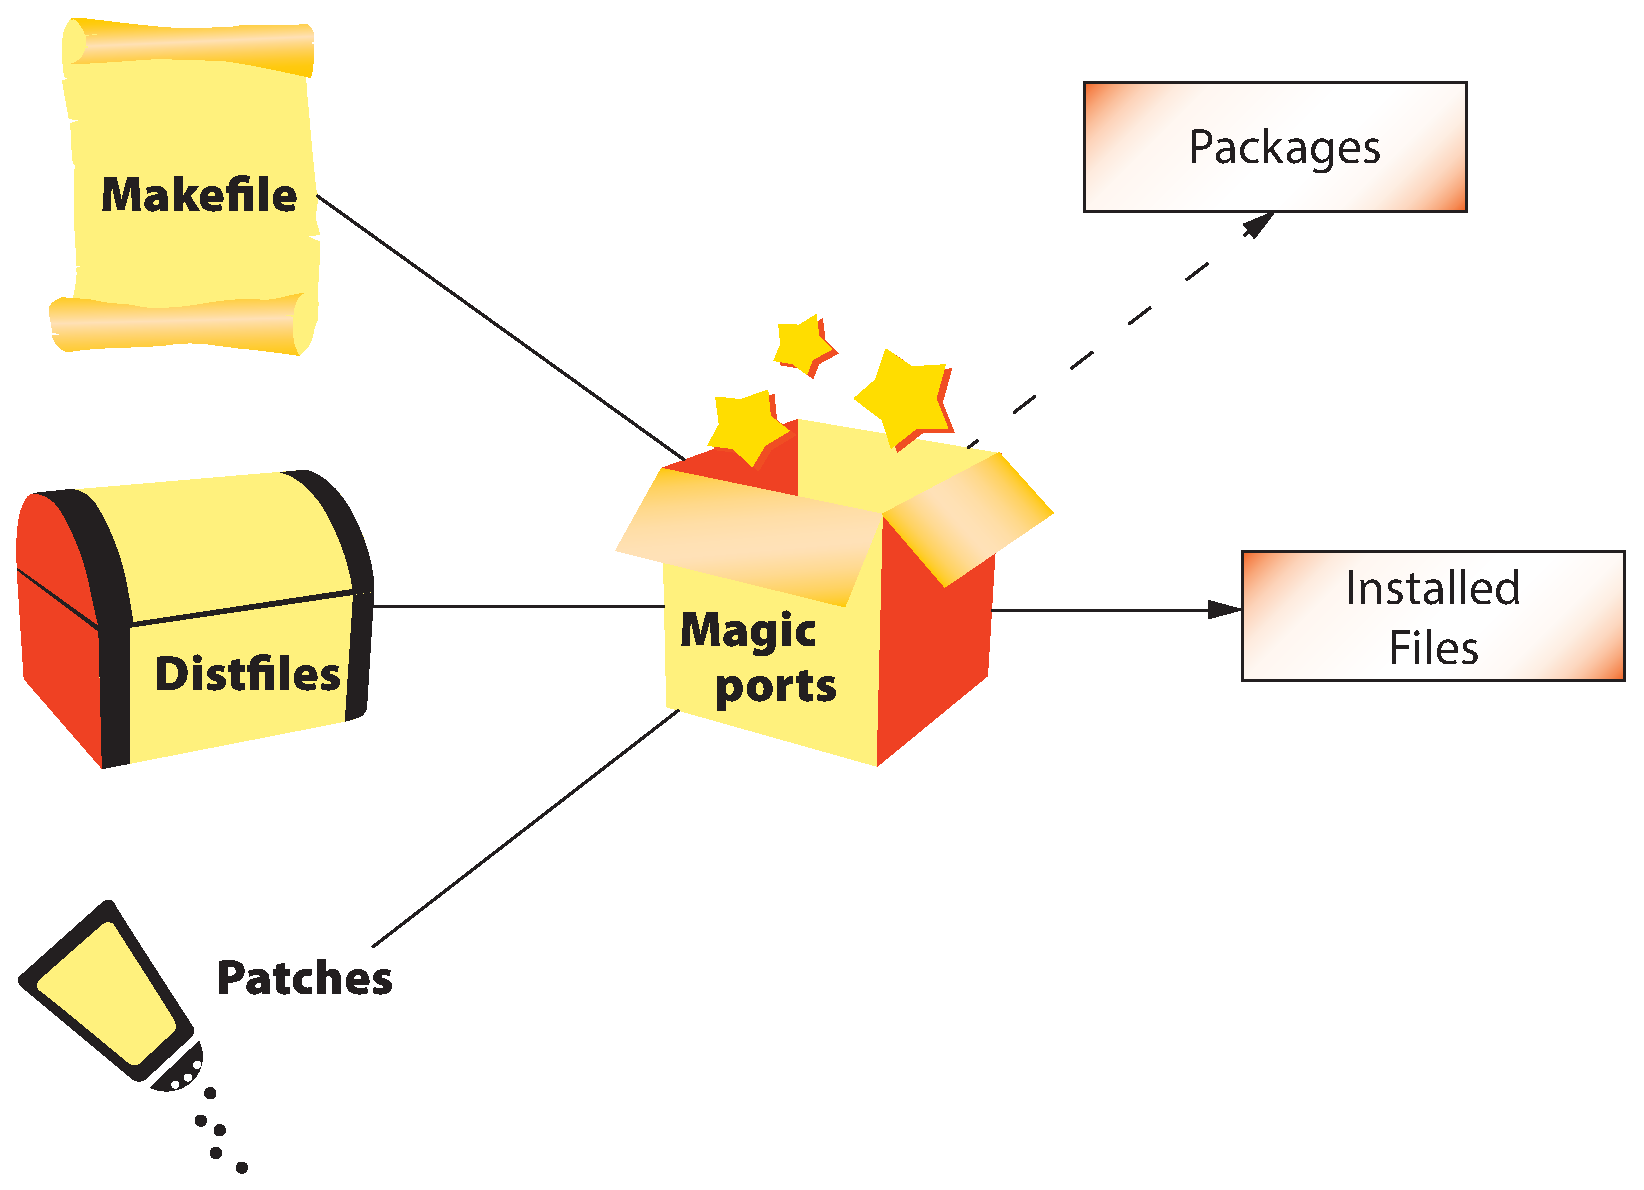
\includegraphics[width=0.95\textwidth]{q1.eps}
%%\end{figure}
%%\end{frame}

\begin{frame}
\frametitle{Planned ports and pkg interaction}
\begin{figure}[h!]
  \centering
  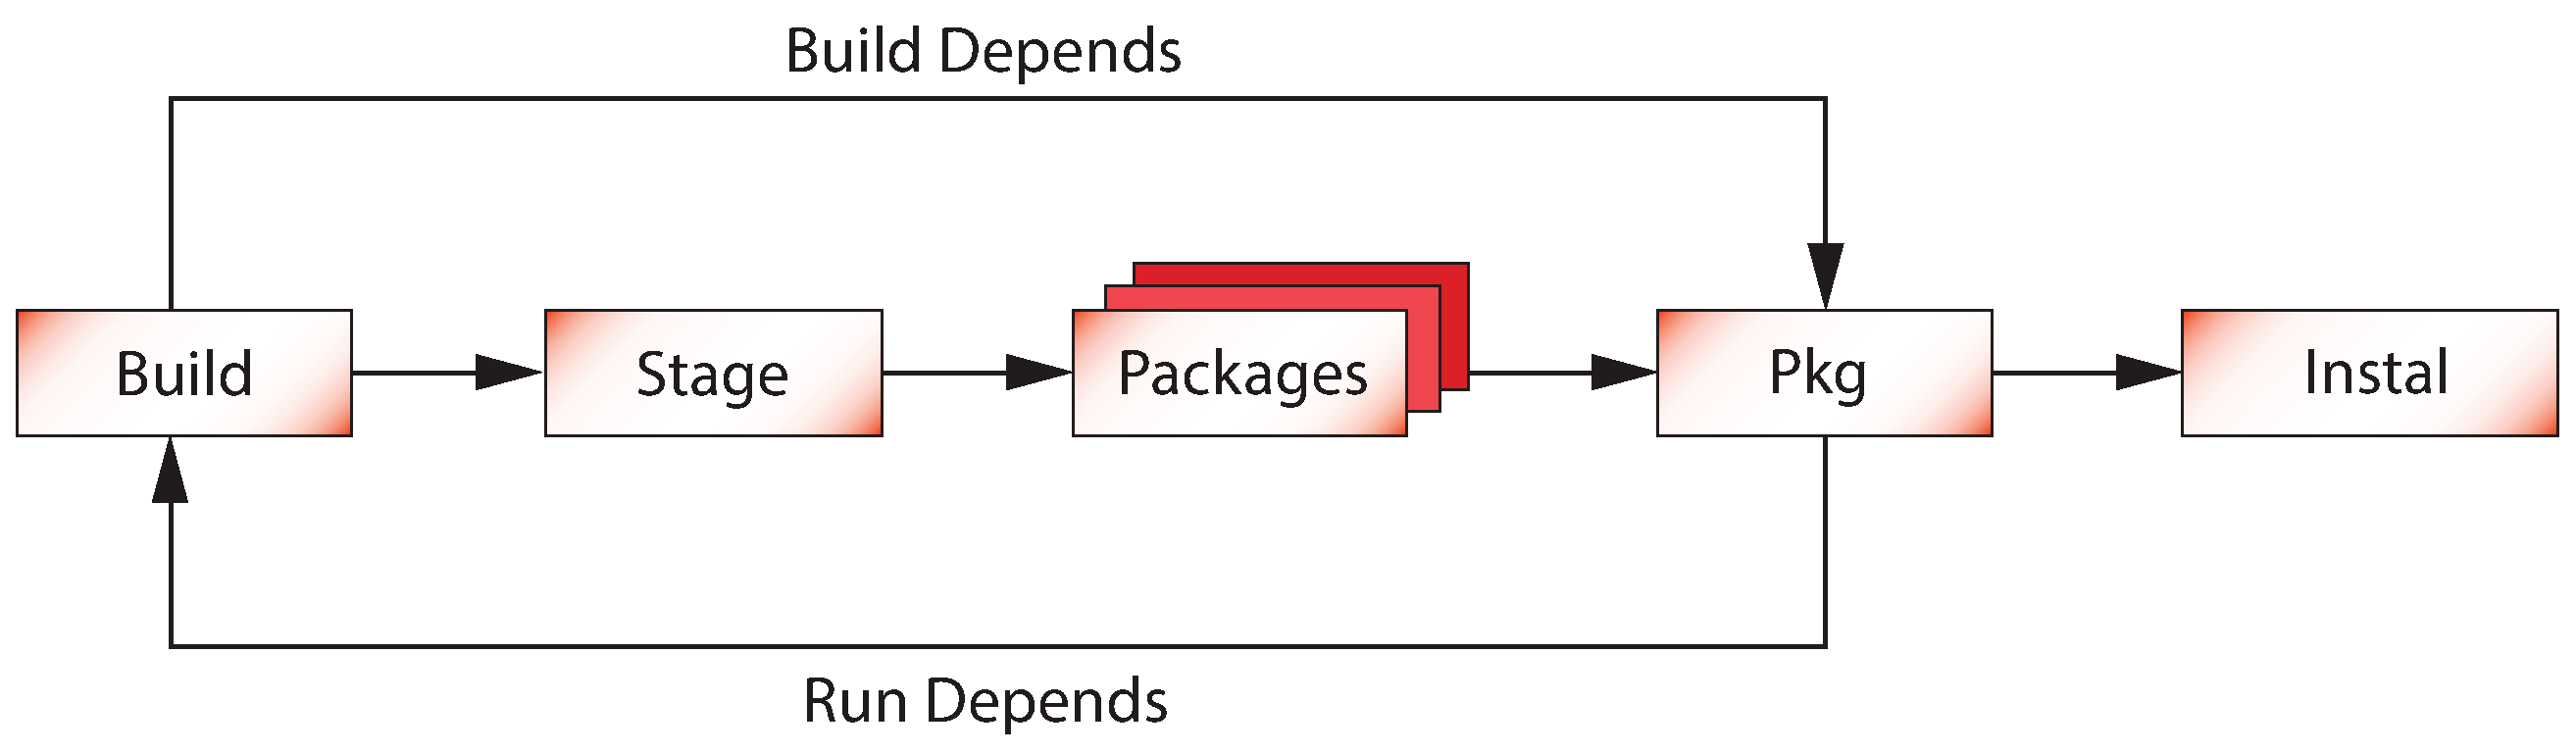
\includegraphics[width=0.99\textwidth]{q2.eps}
\end{figure}
\end{frame}

%%\begin{frame}
%%\frametitle{Repositories creation}
%%\begin{figure}[h!]
%%  \centering
%%  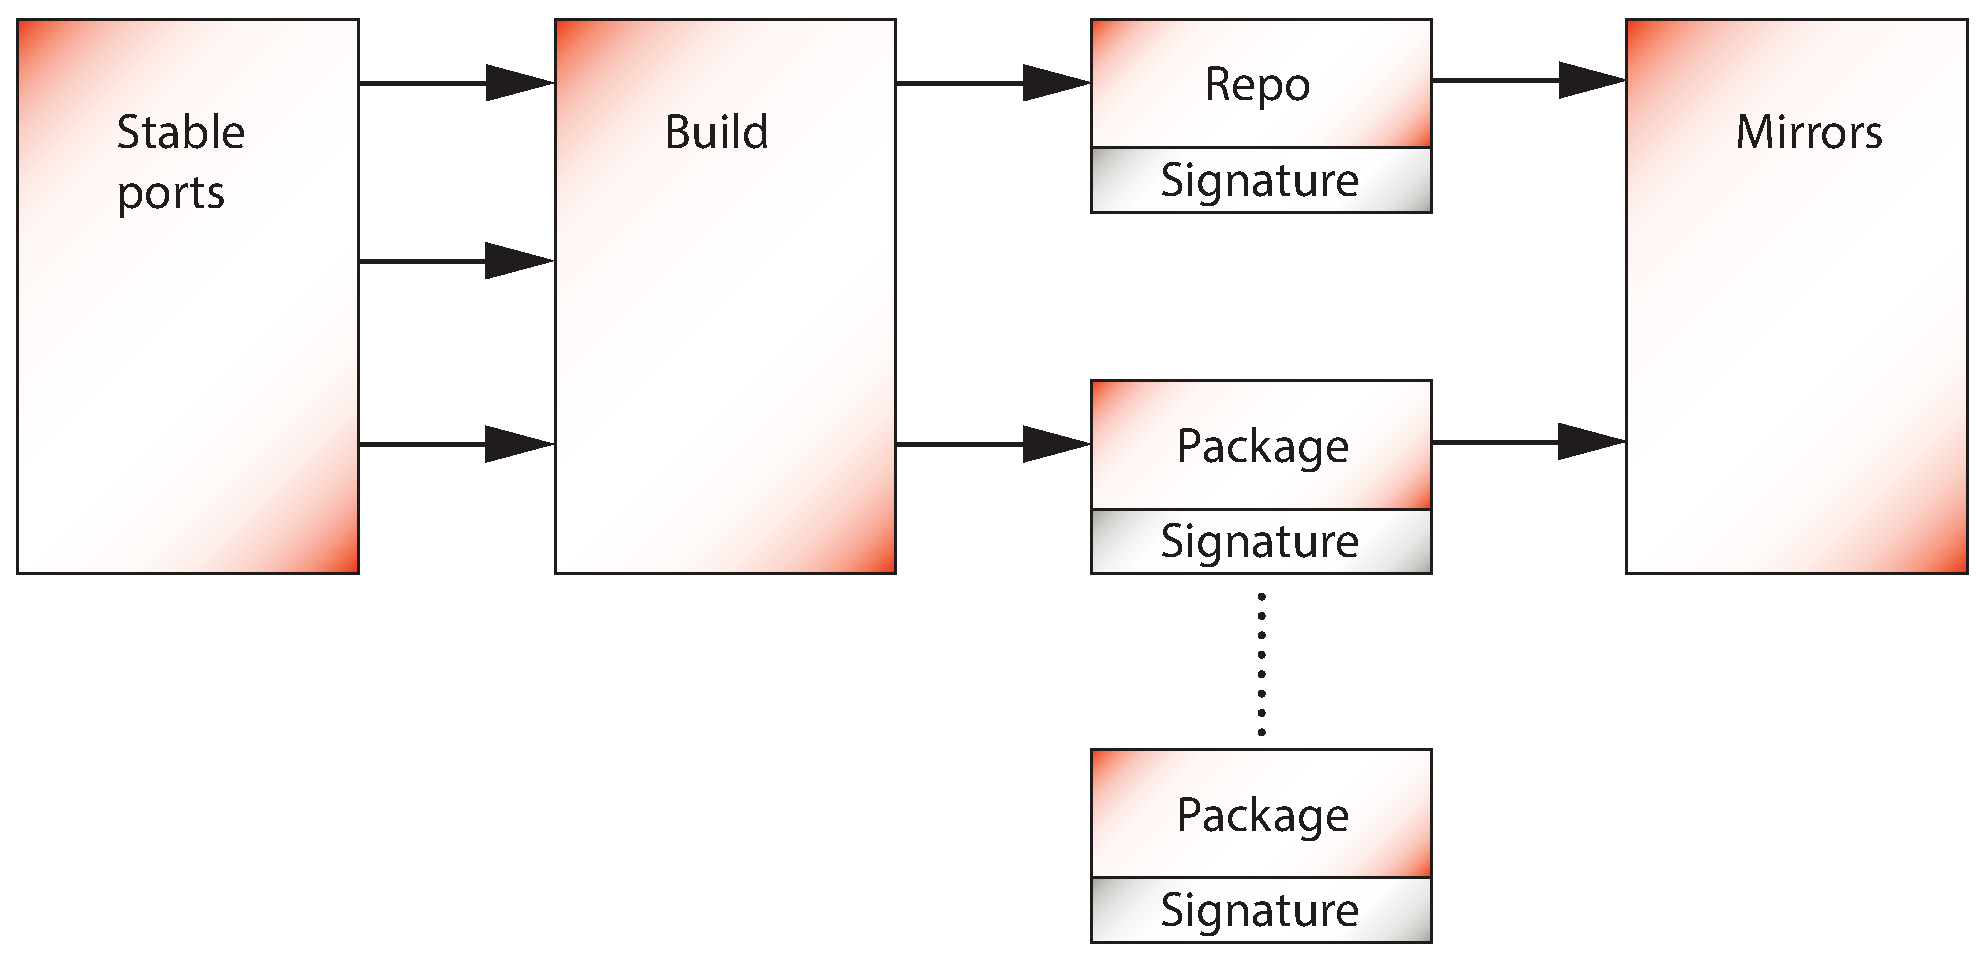
\includegraphics[width=0.95\textwidth]{q3.eps}
%%\end{figure}
%%\end{frame}

%%\begin{frame}
%%\frametitle{The current problems with pkg}
%%\begin{itemize}
%%  \item Legacy ports support (with no staging, for example)
%%  \item Plain dependencies style
%%  \item Naive solver
%%\end{itemize}
%%\end{frame}

\begin{frame}
\frametitle{What is new in pkg 1.3}
\begin{itemize}
  \item New solver that can automatically resolve complex upgrade or install
  scenarios
  \item<2-> Improved security by sandboxing untrusted operations:
  \begin{figure}[h!]
    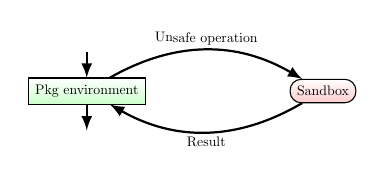
\begin{tikzpicture}[scale=.5, transform shape, auto]
		\tikzstyle{safe_item} = [top color=white,bottom color=green!20, rectangle,
		inner sep=5pt, draw, thin, text centered] 
		\tikzstyle{unsafe_item} = [rounded corners, top color=white,bottom
		color=red!20, rectangle, inner sep=5pt, draw, thin, text centered] 
		\node[safe_item] (safe) at (0, 0) {Pkg environment};
		\node[unsafe_item] (sandbox) at (6, 0) {Sandbox};
		\path[->] 
		(safe) edge [bend left=30,thick,>=latex]
		node[pos=.5,sloped,above]{Unsafe operation} (sandbox) 
		(sandbox) edge [bend left=30, ,thick,>=latex]
		node[pos=.5,sloped,below]{Result} (safe); \draw [->,thick,>=latex] (0,1) --
		(safe); \draw [->,thick,>=latex] (safe) -- (0, -1);
	\end{tikzpicture}
	\end{figure}
	Sandboxing:
	\begin{itemize}
	  \item archives extracting
	  \item vulnxml parsing
	  \item repositories signatures checking and public keys extracting
	\end{itemize}
  \item<3-> Concurrent locking system
\end{itemize}
\end{frame}

\begin{frame}
\frametitle{Pkg architecture}
\begin{figure}[h!]
  \centering
  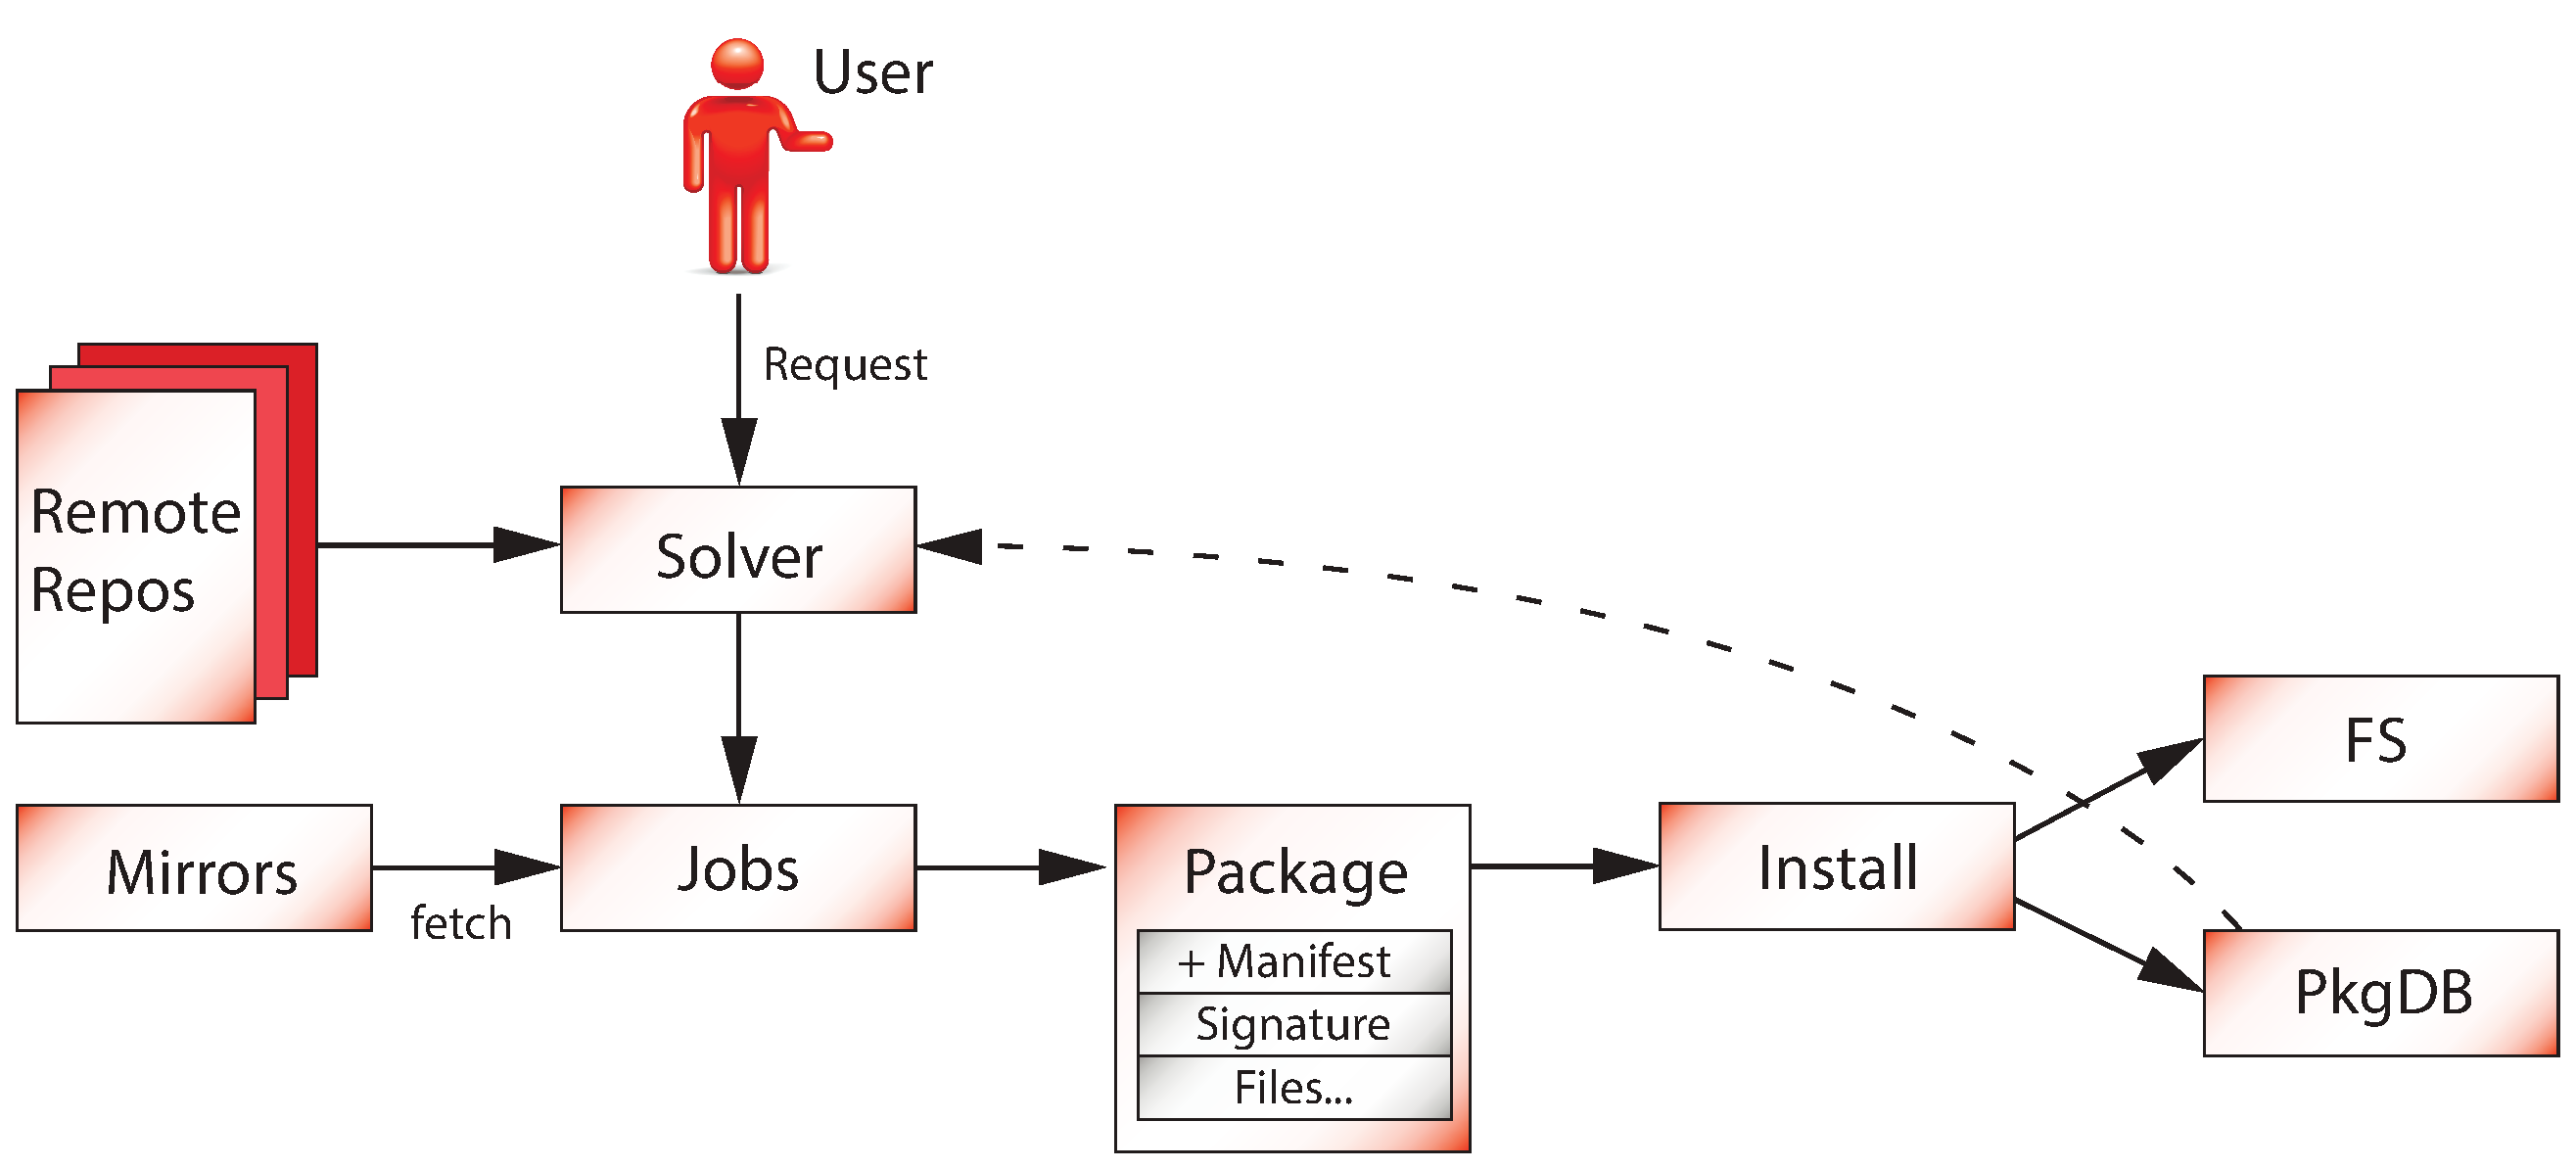
\includegraphics[width=0.95\textwidth]{q4.eps}
\end{figure}
\end{frame}

\begin{frame}
\frametitle{The problems of the old solver in pkg}

\begin{itemize}
\item Absence of conflicts resolving
\item No alternatives support (plain dependencies only)
\item Can perform merely a single task: either install or upgrade or remove
\end{itemize}

\end{frame}

\begin{frame}
\frametitle{Tasks to solve}
\begin{itemize}
  \item Ports renaming: 
  \begin{itemize}
    \item simple:
    \texttt{racket-textual} $\rightarrow$ \texttt{racket-minimal}
    \item splitting/merging: 
    \begin{figure}[h!]
    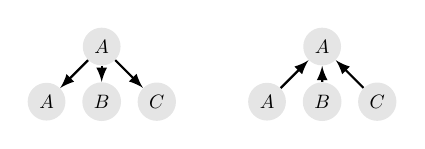
\begin{tikzpicture}[scale=.7, transform shape]
		\tikzstyle{every node} = [circle, fill=gray!20]
		\node (a) at (1, 1) {$A$};
		\node (b) at (0, 0) {$A$};
		\node (c) at (1, 0) {$B$};
		\node (d) at (2, 0) {$C$};
		\foreach \from/\to in {a/b, a/c, a/d}
		\draw [->,thick,>=latex] (\from) -- (\to);
		\node (n1) at (4, 0) {$A$};
		\node (n2) at (5, 0) {$B$};
		\node (n3) at (6, 0) {$C$};
		\node (n0) at (5, 1) {$A$};
		\foreach \from/\to in {n1/n0, n2/n0, n3/n0}
		\draw [->,thick,>=latex] (\from) -- (\to);
	\end{tikzpicture}
	\end{figure}
  \end{itemize}
  \item Ports reorganising:
  	\begin{itemize}
    	\item files moving
    	\item dependencies change
    	\item adding or removing new conflicts
    \end{itemize} 

\end{itemize}
\end{frame}

\begin{frame}
\frametitle{Tasks to solve}
There are another issues to be resolved:
\begin{itemize}
  \item Find conflicts using files list
  \item Set jobs priorities using the following rules:
  \begin{itemize}
    \item install dependencies first
    \item check for reverse dependencies and increase priority
    \item deal with conflicts using the same priority
    \item packages removing reverses the priority order
  \end{itemize}
\end{itemize}
\end{frame}

\begin{frame}
\frametitle{Existing systems}

There are many examples of solvers used in different package management systems,
for example:
\begin{itemize}
  \item 
\includegraphics[width=22pt]{suse.pdf} \hspace{5pt} \texttt{Zypper/SUSE}
  - uses libsolv as the base
  \item 
\includegraphics[width=22pt]{rpm.pdf} \hspace{5pt} \texttt{Yum/RedHat} -
  migrating to libsolv
  \item 
\includegraphics[width=22pt]{puf.pdf} \hspace{5pt}
  \texttt{OpenBSD/pkg\_add} - uses internal solver
  \item 
\includegraphics[width=15pt]{debian.pdf} \hspace{12pt}
  \texttt{Apt/Debian} - uses internal solver
  \item 
\includegraphics[width=15pt]{arch.pdf} \hspace{12pt}
  \texttt{Pacman/Archlinux} - uses internal solver
\end{itemize}

\end{frame}

\begin{frame}[fragile]
\frametitle{External solvers}
To interact with an external solver we have chosen the CUDF format used in the
Mancoosi research project \url{http://mancoosi.org}:
\bigskip
{\small
	\begin{verbatim}
	package: devel/libblah
	version: 1
	depends: x11/libfoo

	package: security/blah
	version: 2
	depends: devel/libblah
	conflicts: security/blah-devel
	
	\end{verbatim}
}
\end{frame}

\begin{frame}
\frametitle{Interaction with external solver}
There are some limitations and incompatibilities with CUDF.
\begin{itemize}
  \item CUDF supports plain integers as versions and we need to convert
  versions twice
  \item There is no support of options in CUDF packages formulas
  \item External solvers are often too complicated and large
  \item CUDF transformation is expensive in terms of performance
\end{itemize}
\end{frame}

\begin{frame}
\frametitle{We need an internal solver!}

Alternatives:
\begin{itemize}
  \item Write own logic of dependencies and conflicts resolution?
  \pause
  \item Use some existing solution?
  \pause
  \item Use some known algorithm?
  \pause
\end{itemize}
\bigskip
{\large Use SAT solver for packages management}
\bigskip
\[
\overbrace{\underbrace{(x_1 \| \neg x_2 \|
x_3)}_{\text{\color{light-gray}Clause}} \& (x_3 \| \neg x_1) \&
(x_2)}^{\text{\color{light-gray}SAT expression}}
\]
\end{frame}

\begin{frame}
\frametitle{Packages universe}
We convert all packages involved to a packages universe of the following
structure:
\begin{figure}[h!]
  \centering
  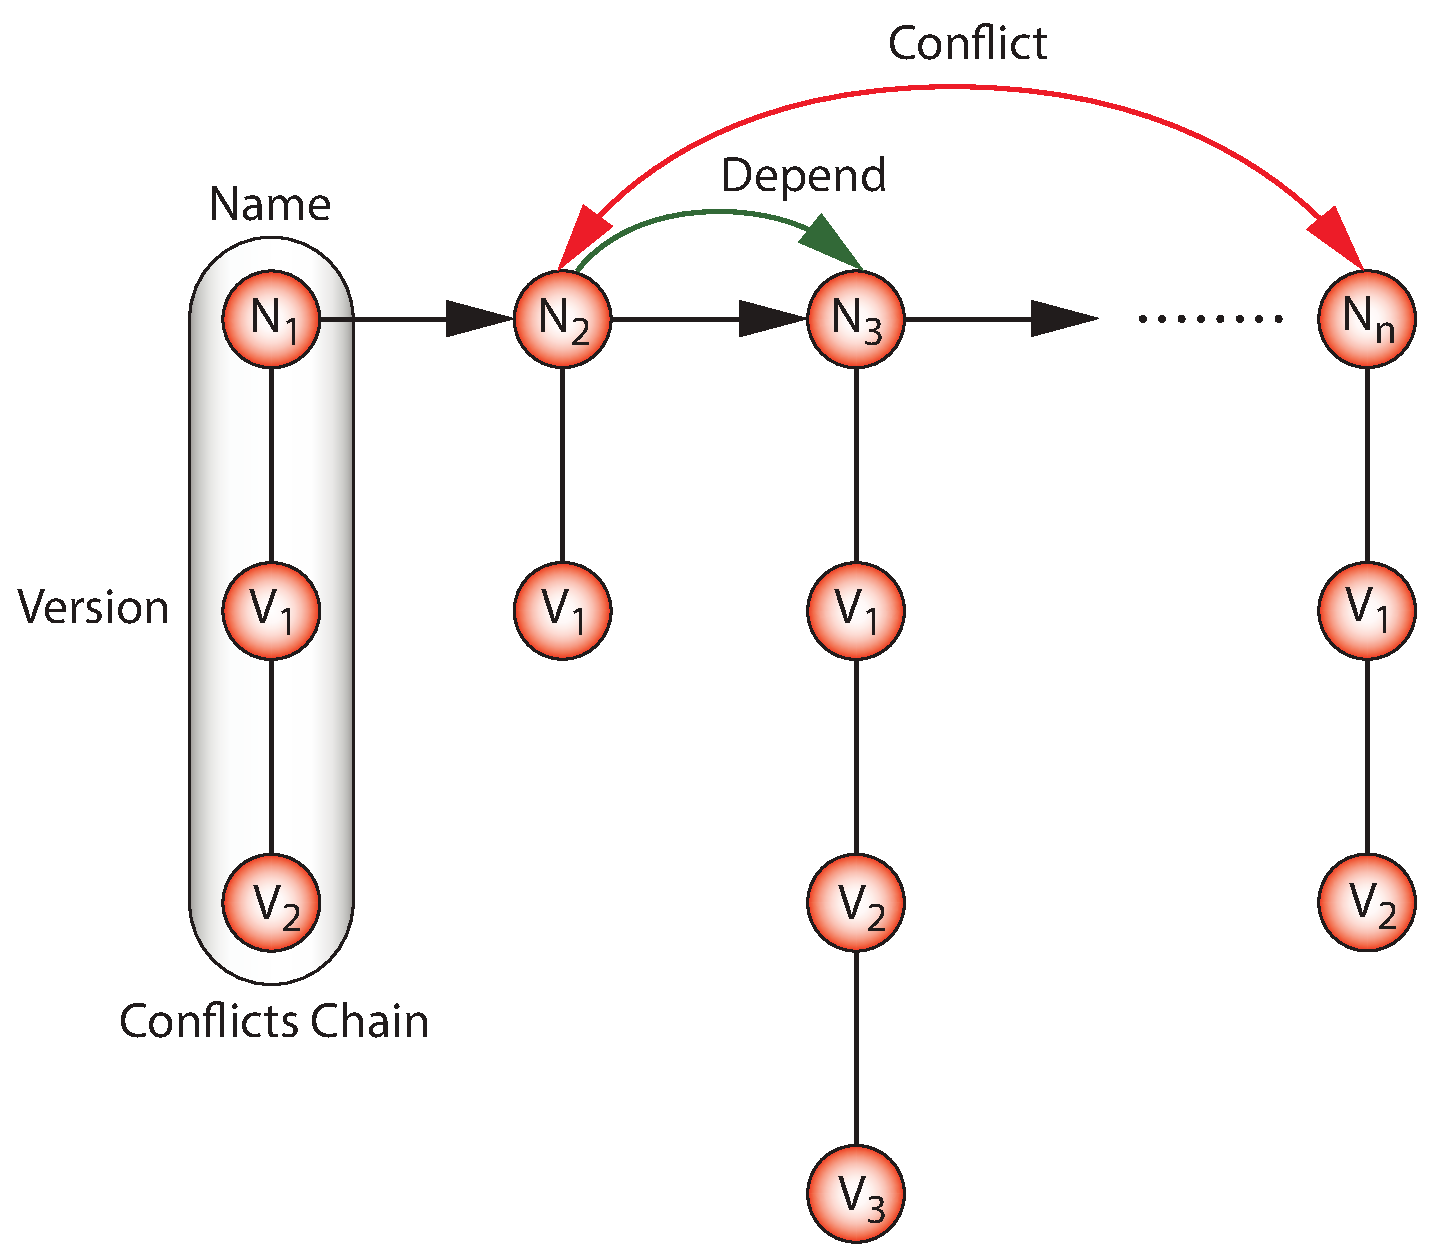
\includegraphics[height=0.7\textheight]{q5.eps}
\end{figure}
\end{frame}

\begin{frame}
\frametitle{Making a SAT problem}
\begin{itemize}
  \item Assign a variable to each package: 
  package A $\to a_1$, package B $\to b_1$
  \item Interpret a request as a set of unary clauses:
  \begin{itemize}
    \item Install/Upgrade package A $\to (a_1)$
    \item Delete package B $\to (\neg b_1)$
  \end{itemize}
  \item Convert dependencies and conflicts to disjuncted clauses
\end{itemize}

\end{frame}

\begin{frame}
\frametitle{Converting dependencies and conflicts}
\begin{itemize}
  \item If package A depends on package B (versions $B_1$ and $B_2$), then we
  can either have package A not installed or any of B installed:
  \bigskip
\[
(\neg A \| B_1 \| B_2)
\]
\pause
  \item If we have a conflict between versions of B ($B_1$, $B_2$ and $B_3$)
 then we ensure that merely one version is installed:
  \bigskip
\[
\underbrace{(\neg B_1 \| \neg B_2) \& (\neg B_1 \| \neg B_3) \& (\neg B_2 \|
\neg B_3)}_{\text{\color{light-gray}Conflicts chain}}
\]
\end{itemize}
\end{frame}

\begin{frame}
\frametitle{The solving of SAT problem}

Some rules to follow to speed up SAT problem solving.
\begin{itemize}
  \item Trivial propagation - solve unary clauses
  \item Unit propagation - solve clauses with only a single unsolved variable
  \item DPLL algorithm backtracking. 
  \item Package specific assumptions.
\end{itemize}
\end{frame}

\begin{frame}
\frametitle{SAT problem propagation}
\begin{itemize}
  \item Trivial propagation - direct install or delete rules
  \bigskip
  \[
  (\neg A \| B) \& \underbrace{(A)}_{\textit{\color{light-gray}true}} \&
  \underbrace{(\neg C)}_{\textit{\color{light-gray}false}} \& (\neg A \| \neg D)
  \]
  \pause
  \item Unit propagation - simple depends and conflicts
  \bigskip
  \[
  \overbracket{\underbrace{(\neg A \| B)}_{B \rightarrow
  \textit{\color{light-gray}true}}}^{\text{\color{light-gray}Dependency}} \&
  \overbrace{(A)}^{\textit{\color{light-gray}true}} \& \overbrace{(\neg
  C)}^{\textit{\color{light-gray}false}} \&
  \overbracket{\underbrace{(\neg A \| \neg D)}_{D \rightarrow
  \textit{\color{light-gray}false}}}^{\text{\color{light-gray}Conflict}}
  \]
  \
\end{itemize}
\end{frame}

\begin{frame}
\frametitle{DPLL algorithm}
DPLL is proved to be one of the efficient algorithms to solve SAT problem (not
the fastest but more simple than alternatives).
\begin{figure}[h!]
  \centering
  \includegraphics<1>[height=0.5\textheight]{dpll1.pdf}
  \includegraphics<2>[height=0.5\textheight]{dpll2.pdf}
  \includegraphics<3>[height=0.5\textheight]{dpll3.pdf}
\end{figure}
\end{frame}

\begin{frame}
\frametitle{Package specific assumptions}
Pure SAT solvers cannot deal with package management as they do not consider
several packages peculiarities:
\begin{itemize}
  \item try to keep installed packages (if no direct conflicts)
  \item do not install packages if they are not needed (but try to upgrade if a
  user has requested upgrade)
\end{itemize}
These options also improve SAT performance providing a good initial assignment.
\end{frame}

%%\begin{frame}
%%\frametitle{Package management task}
%%\begin{itemize}
%%  \item A request is splitted to install/upgrade and delete requests which
%%  could be passed simultaneously to the solver
%%  \item A conflicts between packages are detected with a repository creation
%%  \item All depends, reverse and conflicts of the requested packages are
%%  analyzed and the package universe is created
%%  \item Each package is defined by its name and the digest of significant
%%  fields (version, options and so on)
%%\end{itemize}
%%\end{frame}

\begin{frame}
\frametitle{Solvers and Pkg}
\begin{itemize}
  \item Pkg may pass the formed universe to an external CUDF solver:
  \begin{itemize}
    \item convert versions
    \item format request
    \item parse output
  \end{itemize}
  \item Alternatively the internal SAT solver may be used:
  \begin{itemize}
    \item convert the universe to SAT problem
    \item formulate request
    \item ???
    \item PROFIT
  \end{itemize} 
\end{itemize}
\end{frame}

\begin{frame}
\frametitle{Perspectives}

\begin{itemize}
  \item Using pkg solver for ports management
  \item Better support of multiple repositories
  \item Test different solvers algorithms using CUDF
  \item New dependencies and conflicts format
  \item Provides and alternatives
\end{itemize}
\end{frame}

\begin{frame}
\frametitle{New dependencies format}
\large{\[libblah >= 1.0 +option_1, +option_2 \| libfoo != 1.1\]}
\begin{itemize}
  \item Can depend on normal packages and virtual packages (provides)
  \item Easy to define the concrete dependency versions
  \item Alternative dependencies
\end{itemize}
\begin{figure}[h!]
  \centering
  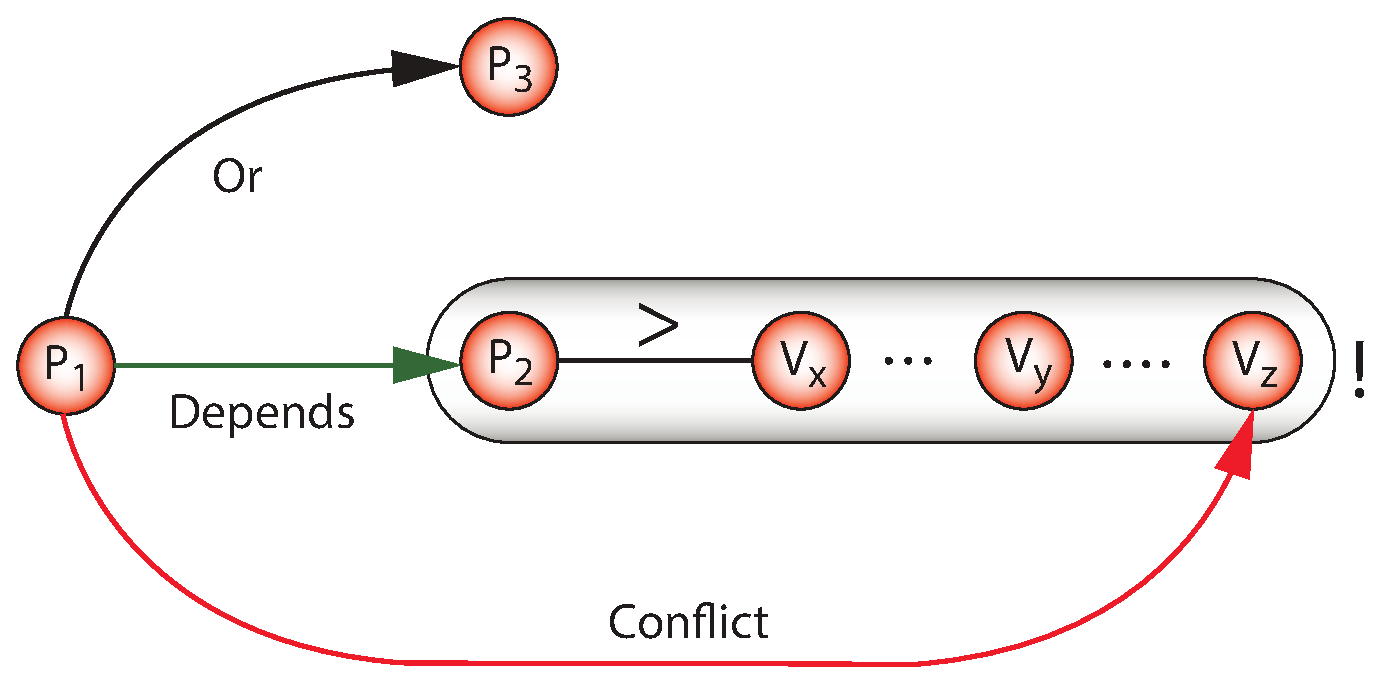
\includegraphics[height=0.3\textheight]{q6.eps}
\end{figure}
\end{frame}

\begin{frame}
\frametitle{Alternatives}
\begin{itemize}
  \item Used to organize packages with the same functionality (e.g.
  web-browser)
  \item May be used to implement virtual dependencies (provides/requires)
\end{itemize}
\begin{figure}[h!]
  \centering
  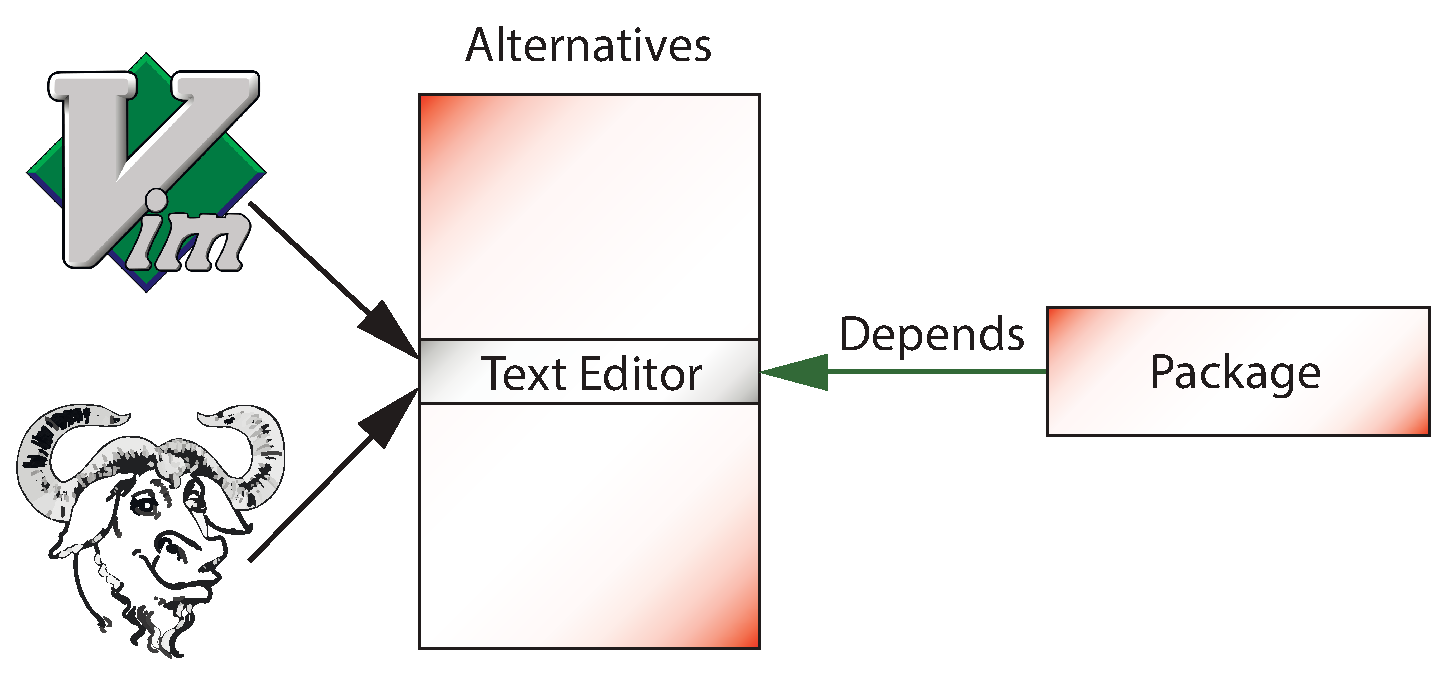
\includegraphics[height=0.4\textheight]{q7.eps}
\end{figure}
\end{frame}

\begin{frame}
\frametitle{Existing issues to be solved prior to 1.3}
\begin{itemize}
  \item A solver cannot find install candidates for non-automatic top level
  packages (those without reverse depends)
  \item Package upgrade is performed improperly (need to rename, install and
  unlink)
  \item Minor issues and crashes
\end{itemize}
\end{frame}

\begin{frame}
\begin{center}

\includegraphics{logo.pdf} \\
\emph{Questions?} \\[4pt]
\url{vsevolod@FreeBSD.org}
\end{center}
\end{frame}

\end{document}
